\documentclass[onecolumn, draftclsnofoot,10pt, compsoc]{IEEEtran}
\usepackage{graphicx}
\usepackage{url}
\usepackage{setspace}
\usepackage{float}
\usepackage{geometry}
\geometry{textheight=9.5in, textwidth=7in}

% 1. Fill in these details
\def \CapstoneTeamName{		Nexusphere}
\def \CapstoneTeamNumber{		48}
\def \GroupMemberOne{			Meghan Mowery}
\def \GroupMemberTwo{			Louis Duvoisin}
\def \GroupMemberThree{			Sarahi Pelayo}
\def \CapstoneProjectName{		A-Frame Live Stream Portal}
\def \CapstoneSponsorCompany{	Oregon State University}
\def \CapstoneSponsorPerson{		Behnam Saeedi}

% 2. Uncomment the appropriate line below so that the document type works
\def \DocType{	%Problem Statement
				%Requirements Document
				%Technology Review
				Design Document
				%Progress Report
				}
			
\newcommand{\NameSigPair}[1]{\par
\makebox[2.75in][r]{#1} \hfil 	\makebox[3.25in]{\makebox[2.25in]{\hrulefill} \hfill		\makebox[.75in]{\hrulefill}}
\par\vspace{-12pt} \textit{\tiny\noindent
\makebox[2.75in]{} \hfil		\makebox[3.25in]{\makebox[2.25in][r]{Signature} \hfill	\makebox[.75in][r]{Date}}}}
% 3. If the document is not to be signed, uncomment the RENEWcommand below
%\renewcommand{\NameSigPair}[1]{#1}

%%%%%%%%%%%%%%%%%%%%%%%%%%%%%%%%%%%%%%%
\begin{document}
\begin{titlepage}
    \pagenumbering{gobble}
    \begin{singlespace}
    	%\includegraphics[height=4cm]{coe_v_spot1}
        \hfill 
        % 4. If you have a logo, use this includegraphics command to put it on the coversheet.
        %\includegraphics[height=4cm]{CompanyLogo}   
        \par\vspace{.2in}
        \centering
        \scshape{
            \huge CS Capstone \DocType \par
            {\large\today}\par
            \vspace{.5in}
            \textbf{\Huge\CapstoneProjectName}\par
            \vfill
            {\large Prepared for}\par
            \Huge \CapstoneSponsorCompany\par
            \vspace{5pt}
            {\Large\NameSigPair{\CapstoneSponsorPerson}\par}
            {\large Prepared by }\par
            Group\CapstoneTeamNumber\par
            % 5. comment out the line below this one if you do not wish to name your team
            \CapstoneTeamName\par 
            \vspace{5pt}
            {\Large
                \NameSigPair{\GroupMemberOne}\par
                \NameSigPair{\GroupMemberTwo}\par
                \NameSigPair{\GroupMemberThree}\par
            }
            \vspace{20pt}
        }
        \begin{abstract}
        % 6. Fill in your abstract    
        	A-Frame Live Stream Portal is a project that will be used to bring families closer together, even when adversity keeps them apart. 
        	The main parts of this report are the introduction, design viewpoints, and design views.
        \end{abstract}   	 
    \end{singlespace}
\end{titlepage}
\newpage
\pagenumbering{arabic}
\tableofcontents

% 7. uncomment this (if applicable). Consider adding a page break.
\listoffigures
\listoftables
\clearpage

% 8. now you write!
\begin{center}
 \begin{tabular}{||p{1cm} p{7cm} p{7cm}||} 
 \hline
 Section & Original & New\\ [.5ex] 
 \hline\hline
 1.3 & Had 720p as resolution & Lowered to 480p\\
 \hline
  1.3 & Microphone was originally going to be it's own separate pi & Microphones now attached to all pis\\
   \hline
  3.2 & Had one microphone & Now uses three microphones\\
  \hline
  3.3.1 & Referenced using a UML diagram & Removed references\\ 
  \hline
  3.3.2 & Referenced using a UML diagram & Removed references\\ 
  \hline
  3.3.3 & Microprocessor section & Removed section, no longer using microprocessor  \\
  \hline
  3.3.3/4 & Mentioned using 1 microphone & Now using 3 microphones \\
    \hline
 3.4.1 & Mentioned microprocessor & Removed microprocessor reference and added a microphone per pi \\
  \hline
 3.4.1 & VLC was going to be used for streaming & Picam and a node plugin were used instead \\ 
 \hline
 3.4.1 & MJPEG was the original file format & HLS is what was used\\ 
 \hline
 3.4.2 & 360 video camera was going to be purchased & The raspberry pi camera module with a 360 degree lens attachment was used\\
 \hline
 3.4.3 & Section talking about microprocessor & Removed section \\ 
 \hline
 3.4.3/4 & Microphone design was using one microphone and a microprocessor to merge audio & New design has a microphone on every pi creating a stream with audio \\ 
 \hline
 3.4.4/5 & Section references the ad hoc network & Revisions regarding the ad hoc network\\
 \hline
 Figures & Old pictures of prototypes & New pictures of the current appearance of the website\\[1ex] 
 \hline
\end{tabular}
\end{center}

\section{Introduction}
    \subsection{Purpose}
    The purpose of this document is to describe the different physical aspects of this project.
    By describing the aspect of the project in detail, it will be easier to formulate a plan to complete the project.
    This includes describing the design concerns, views, and viewpoints of this project.
    
    \subsection{Scope}
    This document will cover all aspects of the project, including the hardware and software development.
    This document also includes various images related to the system's user interface and design.
    
    \subsection{Context}
    A-frame live stream portal is a project that will utilize various technologies to allow the stakeholder's family to view the stakeholder's wedding live.
    The project consists of three cameras, two regular view and one 360 view which will be live streaming the wedding at 480p and 30fps. 
    Each raspberry pi will have a microphone attached which will provide audio for the stream coming from that pi.
    Finally, the web portal that will be created will be used by both the stakeholder and the stakeholder's family.
    The stakeholder will have access to an admin page where they can move, add, or delete cameras and microphones as well as change the displayed venue map.
    The users will be able to select any of the available cameras on the map to view the wedding ceremony.
    This way the family of the stakeholder will be able to experience the wedding as if they were there themselves.
    
\begin{thebibliography}{}
\bibitem{IEEEhowto:AFrame}
[online] A-Frame. Available at: https://aframe.io/ [Accessed 2 Nov. 2018].

\bibitem{IEEEhowto:Audio}
Hills, Mark (December 2017). trx: Realtime audio over IP.
[online] Available at: http://www.pogo.org.uk/~mark/trx/
[Accessed 27 Nov. 2018]

\bibitem{IEEEhowto:Microprocessor-video-streaming}
Roberts, L. (2018). Raspberry Pi MJPEG at ~30fps - lewisroberts.com. [online] lewisroberts.com. Available at: https://www.lewisroberts.com/2015/05/15/raspberry-pi-mjpeg-at-30fps/ [Accessed 28 Nov. 2018].
\bibitem{IEEEhowto:ad-hoc}
Pinola, M. (2018). Features and Uses of an Ad Hoc Wireless Network. [online] Lifewire. Available at: https://www.lifewire.com/what-is-an-ad-hoc-wireless-network-2377409 [Accessed 28 Nov. 2018].
\end{thebibliography}

\section{Glossary}
%\begin{table}[H]
%\caption{Glossary}
\label{tab:Glossary}
\begin{tabular}{l5}
         Access Token/Login Key & Sequence of characters used for authentication \\
         A-Frame & The web framework that will be used for 360 video \\
         CSS & Cascading Style Sheet\\
         Fps & Frames Per Second \\ 
         Jpeg & Joint Photographic Experts Group (image file format) \\ 
         Mbps & Mega bits per second \\
         Mjpeg & Motion Joint Photographic Experts Group 720p \& Progressive video format with 720 horizontal lines\\
         Png & Portable Network Graphics (image file format) \\
         TCP & Transmission Control Protocol\\
         UDP & User Datagram Protocol \\
         USB & Universal Serial Bus\\
         UI & User interface \\
         Server & The computer hosting the website and receiving the video\\ 
         Web Portal & A website that displays information from multiple external sources \\ 
         Wi-fi & Wireless Fidelity
\end{tabular}
%\end{table}

\section{Body}

    \subsection{Identified design stakeholders}
    The stakeholders for this project are Behnam and Jenna Saeedi.
    
    \subsection{Identified design concerns}
    This project will require both a user interface (UI) and technological implementation.
    The web portal will have two different interfaces, admin and user, and will be simple and easy to understand.
    The technologies used for this project will be two video cameras, one 360 degree video camera, three microphones, and multiple raspberry pis.
    
    \subsection{Selected design viewpoints}
    %identifies the design concerns to be focused upon within its view and selects the design languages used to record that design view
        \subsubsection{Normal Video}
        The video needs to be live streamed from the wedding to the stakeholder's family.
        This video will ideally stream at 1080p and 30fps with a minimum of 480p, still with 30fps.
        The stream can be interacted with by the stakeholder's family.
        The camera will need to last the entire wedding ceremony.
        
        \subsubsection{360 Video}
        The 360 video needs to be live streamed from the wedding to the stakeholder's family.
        This video will ideally stream at 1080p and 30fps, and can be interacted with by the stakeholder's family.
        The camera will need to have a strong enough battery so it can last the entire wedding ceremony.
        
        %\subsubsection{Microprocessor}
        %The microprocessor has to have the capability to stream either the regular or 360 degree video to the web portal without any significant delays. 
        
        \subsubsection{Microphone}
        To get the full experience of the wedding for the family of the client along with streaming video there will be audio to accompany it. The system’s design includes three cameras and three microphones. Because each raspberry pi will have it's own microphone attached, each stream will have it's own audio feed.  
        A subsystem is a camera or microphone connected to a microprocessor. 
        The goal of the microphones are to record and stream audio so it can be projected over the each video broadcast coming from the other raspberry pis. 
        
        \subsubsection{Web Server Architecture}
        The web server architecture must be designed so all the video and audio streams from the four subsystems can be sent to a web server. 
        The network design must allow for subsystem independence, meaning that if one of the cameras fails the others must remain unaffected.  
        %probably have images showing how our technologies will be used
        %IE: front end/back end/hardware
        %UI & Video Player/Web Host/Streaming device & Camera
        
        \subsubsection{Desktop UI}
        The user interface needs to be designed in a way that is simple to use for both the client and the end user. 
        A custom website will be designed. The website's UI will be tailored with input from the client.  
        The design will go through a feedback process where a prototype will be presented to the client, and the client will leave feedback as they see fit. 
        After the client's feedback the prototype will be updated and shown to the client again. 
        The web page will require users to login to view the venue map, and be able to select a device from a camera to watch the wedding. 
        Users will also need to be able to return back to the venue map and select a different device. 
        There will also be an admin view from which the client can add, move, and remove cameras, as well as upload a new venue map.
        
        \subsubsection{Mobile UI}
        In addition to working on desktop, the website will also need to be usable on mobile devices. 
        All functionality available in the desktop UI must be available for mobile.
        
    \subsection{Design views}
    %Each view addresses a specific set of design concerns of the stakeholders
        \subsubsection{Normal Video}
        Video in normal view will contain two subsystems consisting of a raspberry pi camera module and microphone. 
        The module with be connected to the raspberry pi's camera port using a ribbon cable. 
        For video streaming, the design will need a video media player. 
        Picam will be used to record the stream and a node app will act as the server for the stream because it has several options to customize the stream so it can meet the requirements of a minimum of 480p with 30fps. 
        The video will be in HLS format and adjusted to a reasonable bit rate at will depend on the strength of the venue's Wi-Fi. 
        
        \subsubsection{360 Video}
        The 360 video stream will be done with a basic raspberry pi camera module and an additional attachment that is used for streaming 360 video on iPhone, the user will connect the pi and operate it the same way they would operate the regular videos on the raspberry pi.
        The video will then be streamed to the website using A-Frame.
        The team chose to upload the video directly to the website instead of going through another format such as YouTube or Facebook.
        
        \subsubsection{Microphone}
        The best design approach selected will be to have a microphone connected to each raspberry pi.  
        The independence of the mentioned design choices meets the need for safeguarding from total system failure as a result from one competent or subsystem failure.
        A USB microphone will be used on each raspberry pi 3 to record the audio used for each stream. 
        USB microphones have easy interfaces meaning that it can be inserted into any USB port. 
        The audio will be streamed with picam, which captures both audio and video from the attached pi. 

        
        \subsubsection{Web Server Architecture}
        Each of the microprocessors need to have a built-in wifi module to be able to connect to the internet. 
        The network will consists of three subsystems, two normal video, and one 360. 
        Each microprocessor will send captured video and audio to the web server directly using the venue internet. 
        The raspberry pi from a will have the IP address of the venues router then the router will port forward to the pi. The video will be port forwarded from each of raspberry pi to the router then sent over to the OSU server.
        \vspace{1cm}
        \begin{figure}[H]
            \centering
            \includegraphics[scale=0.5]{Images/server-architecture.png}
            \centering\caption{System Architecture}
            \label{fig:Architecture}
        \end{figure}
        \pagebreak
        
        \subsubsection{Desktop UI}
        Figure \ref{fig:Login} is the login page of the system's website. Users will be given a login key which they will input. When the user's enter the correct key they will be taken to the main page, Figure \ref{fig:User}. The main page is where users will be able to select which stream they want to watch. The main page also has an admin view shown in Figure \ref{fig:Admin}. The client will be able to get to admin view by logging in with a separate login key for the admin login. The buttons will open menus that will allow the client to perform the labeled action (ex: add a device, remove a device, etc). In both admin and normal user mode clicking on a camera will redirect the user to that camera's stream viewable in Figure \ref{fig:Video}. The video page will be the same for both normal and 360 video.
        \vspace{1cm}
        \begin{figure}[H]
            \centering
            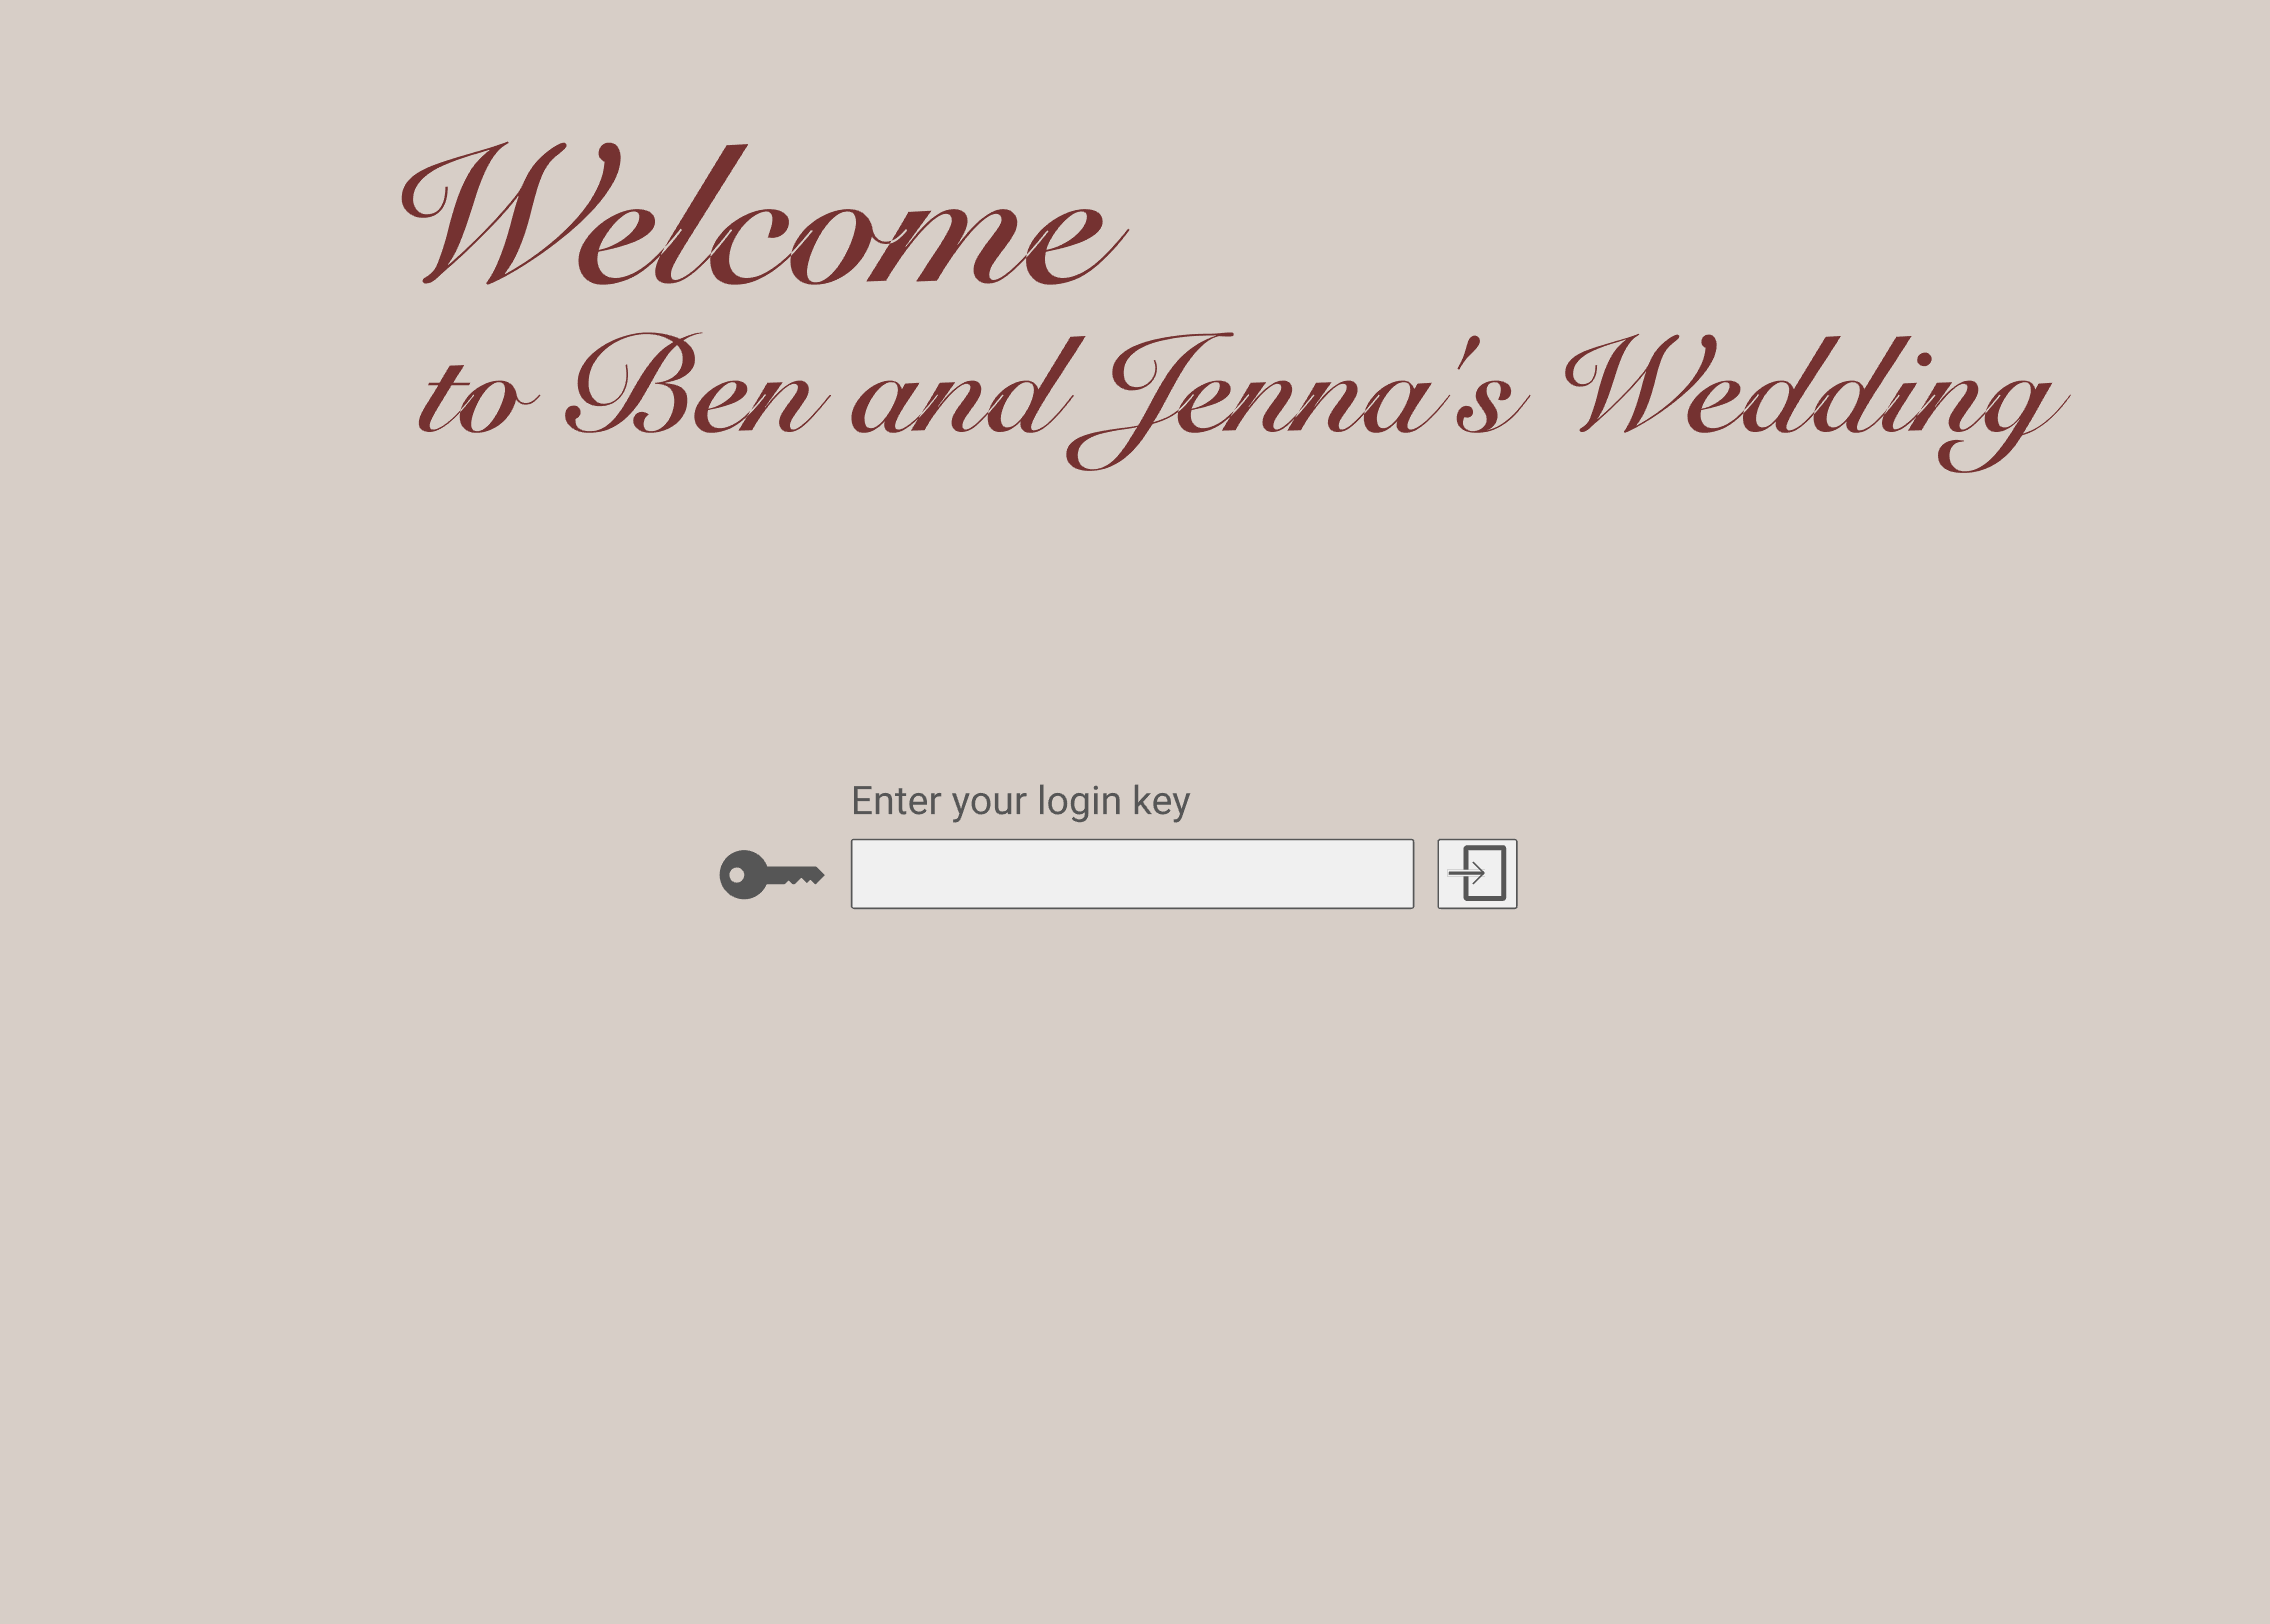
\includegraphics[scale=0.4]{Images/desktop-login.png}
            \centering\caption{Login Page}
            \label{fig:Login}
        \end{figure}
        
        \begin{figure}[H]
            \centering
            \includegraphics[scale=0.17]{Images/website_pics/desktop-viewer.png}
            \centering\caption{User View}
            \label{fig:User}
        \end{figure}
        \begin{figure}[H]
            \centering
            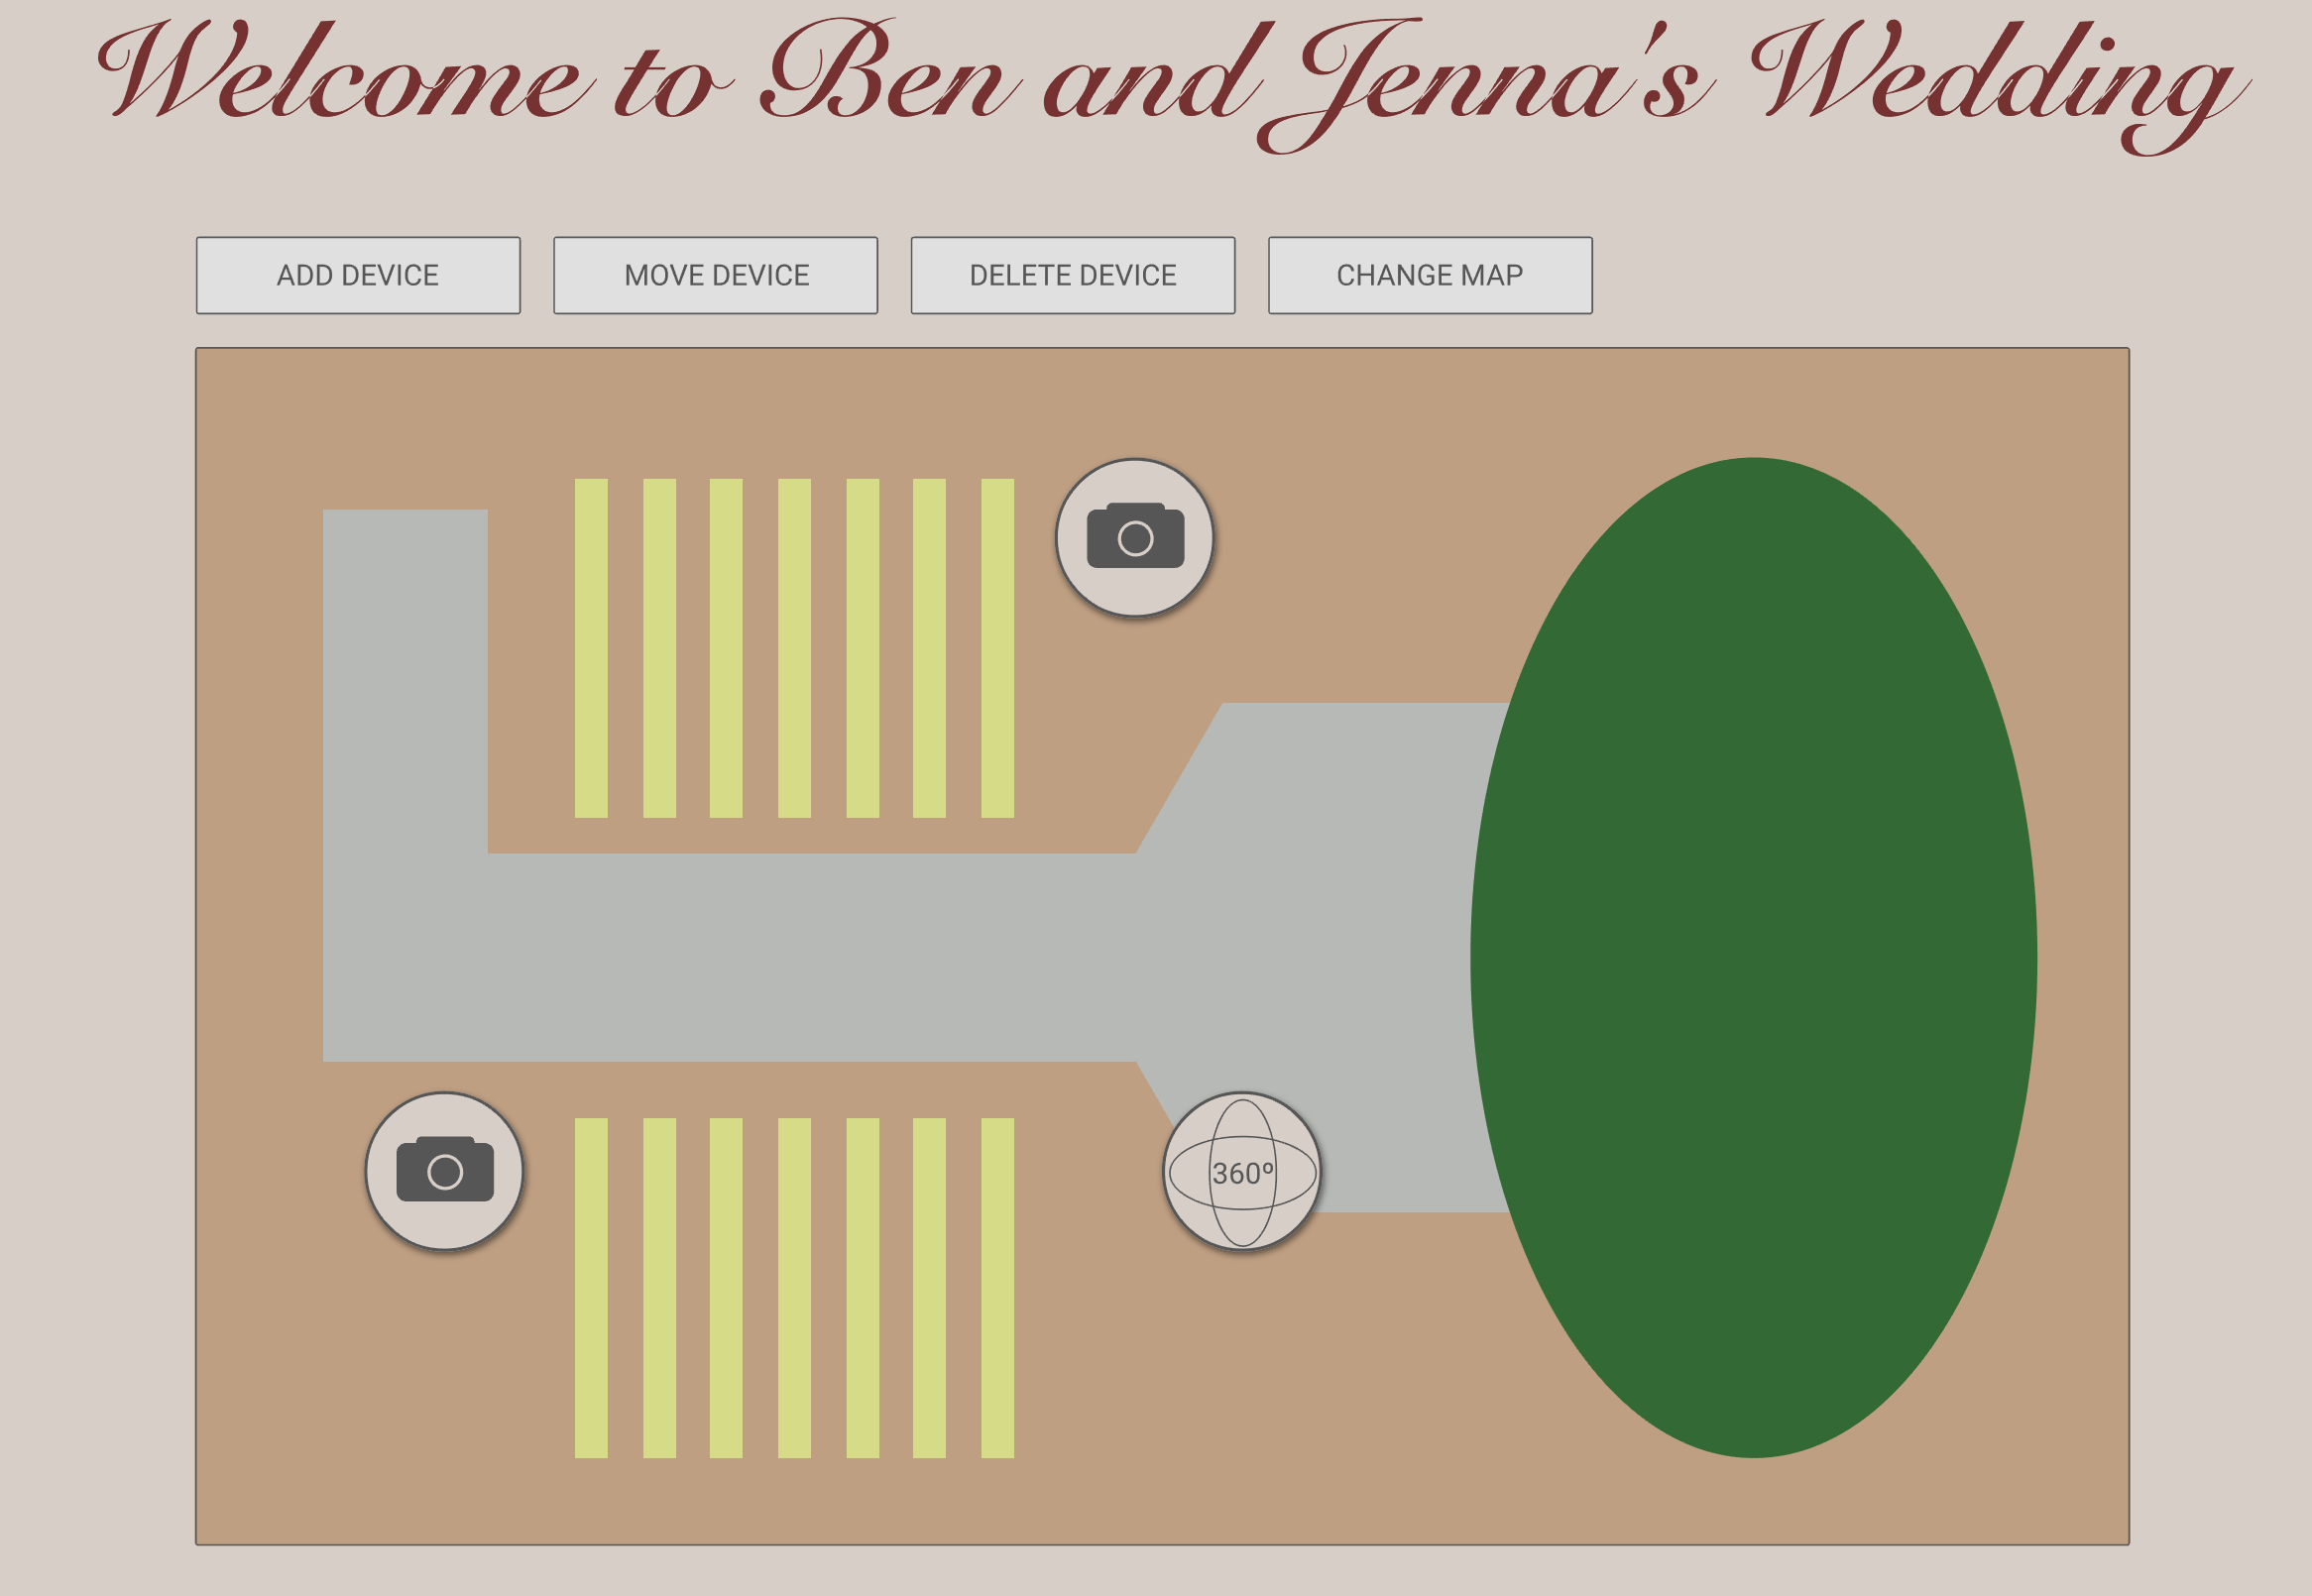
\includegraphics[scale=0.17]{Images/website_pics/desktop-admin.png}
            \centering\caption{Admin View}
            \label{fig:Admin}
        \end{figure}
        
        \begin{figure}[H]
            \centering
            \includegraphics[scale=0.35]{Images/website_pics/video_image.png}
            \centering\caption{Video Page}
            \label{fig:Video}
        \end{figure}
        
         \begin{figure}[H]
            \centering
            \includegraphics[scale=0.4]{Images/website_pics/change_map.PNG}
            \centering\caption{Change Map Image}
            \label{fig:Map}
        \end{figure}
        
         \begin{figure}[H]
            \centering
            \includegraphics[scale=0.4]{Images/website_pics/add_device.PNG}
            \centering\caption{Add Device}
            \label{fig:Add}
        \end{figure}
        
         \begin{figure}[H]
            \centering
            \includegraphics[scale=0.4]{Images/website_pics/delete_device.PNG}
            \centering\caption{Delete Device}
            \label{fig:Delete}
        \end{figure}
        
        \begin{figure}[H]
            \centering
            \includegraphics[scale=0.4]{Images/website_pics/move_select.PNG}
            \centering\caption{Move Device}
            \label{fig:Move}
        \end{figure}
        
        \subsubsection{Mobile UI}
        The mobile UI will contain the same pages as the desktop UI and have all of the same functionality. The system's CSS will be written such that the user will be loading what would be the same page both on desktop and mobile, but the page's components for the mobile view will be oriented differently. 
    %MOBILE pictures    
       
        \begin{figure}
            \centering
            \includegraphics[scale=0.3]{Images/website_pics/mobile/login_mobile.jpg}
            \centering\caption{Mobile Login}
            \label{fig:MLogin}
        \end{figure}
        
        \begin{figure}
            \centering
            \includegraphics[scale=0.3]{Images/website_pics/mobile/viewer_mobile.jpg}
            \centering\caption{Mobile User View}
            \label{fig:MUser}
        \end{figure}
        
        \begin{figure}
            \centering
            \includegraphics[scale=0.3]{Images/website_pics/mobile/admin_mobile.jpg}
            \centering\caption{Mobile Admin View}
            \label{fig:MAdmin}
        \end{figure}

        \begin{figure}
            \centering
            \includegraphics[scale=0.3]{Images/website_pics/mobile/video_mobile.jpg}
            \centering\caption{Mobile Video Page}
            \label{fig:MVideo}
        \end{figure}



\end{document}